\section{PID-Regler nach Kuhn}
Nach den Einstellregeln von Kuhn ist der PID-Regler wie folgt zu dimensionieren
\[
	\begin{array}{l c l}
		K_p & = & \frac{2}{K_g} \\
		T_i & = & 0.8 \cdot T_\Sigma \\
		T_d & = & 0.194 \cdot T_\Sigma
	\end{array}
\]
Die Zeitkonstante $T_\Sigma$ ist für die vorliegende Übertragungsfunktion
\[
	T_\Sigma = 2 \cdot T_1 + T_d
\]


\subsection{$G_1(s)$}
Die Übertragungsfunktion $G_1(s)$ ist definiert als
\[
	G_1(s)
	= \frac{K_g}{(T_1 \cdot s + 1)
		\cdot (T_1 \cdot s + 1)}
		\cdot e^{-T_d \cdot s}
	\qquad ,T_1 = 0.1468 \si{\second}
	\quad ,T_d = 0.035 \si{\second}
	\quad ,K_g = 245.5 \si[per-mode=fraction]{\per\volt\per\minute}
\]
Mit den oben genannten Einstellregeln ergeben sich die folgenden Werte
\[
	\begin{array}{l c l}
		K_p & = & 0.008147 \si[per-mode=fraction]{\volt\per\minute} \\
		T_i & = & 0.26288 \si{\second} \\
		T_d & = & 0.06375 \si{\second} 
	\end{array}
\]

\subsection{$G_2(s)$}
Die Übertragungsfunktion $G_2(s)$ ist definiert als
\[
	G_s(s)
	= \frac{K_g}{(T_1 \cdot s + 1)
		\cdot (T_1 \cdot s + 1)}
		\cdot e^{-T_d \cdot s}
	\qquad ,T_1 = 0.1015 \si{\second}
	\quad ,T_d = 0.045 \si{\second}
	\quad ,K_g = 150.5 \si[per-mode=fraction]{\per\volt\per\minute}
\]
Mit den oben genannten Einstellregeln ergeben sich die folgenden Werte
\[
	\begin{array}{l c l}
		K_p & = & 0.01329 \si[per-mode=fraction]{\volt\per\minute} \\
		T_i & = & 0.1984 \si{\second} \\
		T_d & = & 0.048112 \si{\second} 
	\end{array}
\]

\subsection{Messdaten}

\begin{figure}[h!]
	\centering
	\begin{subfigure}{0.475\textwidth}
		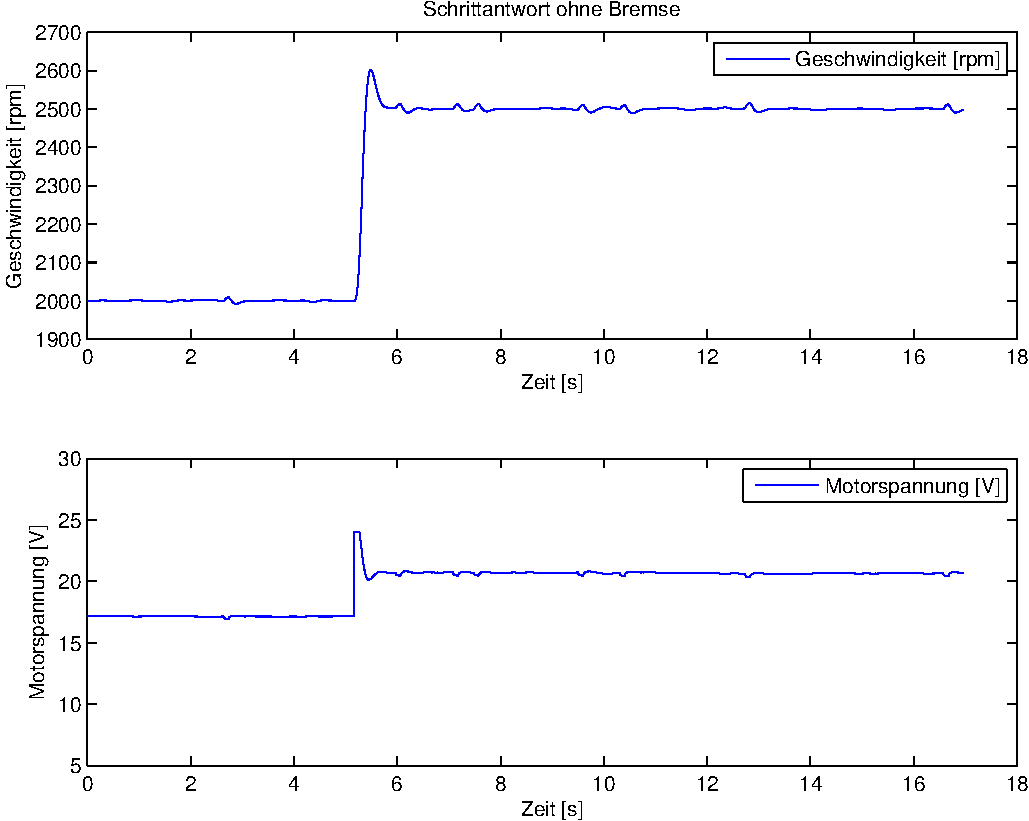
\includegraphics[width=1\textwidth]{09/step_noload.pdf}
		\caption{Ohne Bremse ($\alpha = 0$)}
	\end{subfigure}
	\hfill{}
	\begin{subfigure}{0.475\textwidth}
		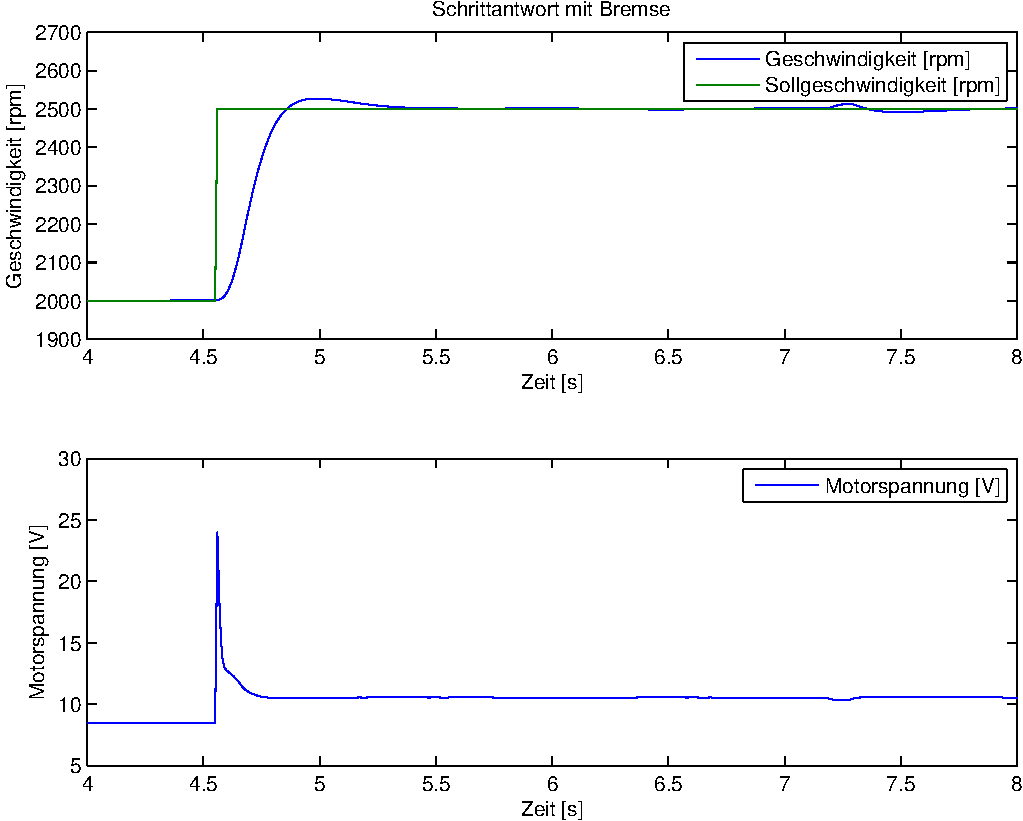
\includegraphics[width=1\textwidth]{09/step_load.pdf}
		\caption{Ohne Bremse ($\alpha = 0$)}
	\end{subfigure}
	\caption{Sprungantworten des PID-Reglers nach Kuhn}
\end{figure}


\begin{table}[h!]
	\centering
	\begin{tabular}{l c c c c}
		Eigenschaft
			& Spezifikation
			& $\alpha = 0$
			& $\alpha = 0.5$
			& Einheit \\
		\hline
		Genauigkeit (mean)
			& 100
			& 100
			& 100
			& \% \\
		Anregelzeit (0-99\%)
			& $0.8$
			& 0.22
			& 0.3
			& $\si{\second}$ \\
		Überschwingen
			& $15$
			& 20.45 
			& 5.41 
			& \% \\
		Einschwingzeit
			& $2$
			& n.a. 
			& n.a.
			& $\si{\second}$ \\
	\end{tabular}
\end{table}
